Como podemos observar existen numerosos errores en nuestro proyecto, ello es debido a la falta de las librerías de Torque y Village. Las añadimos desde las siguientes direcciones:

\begin{lstlisting}
coches\torque-3.3\lib
\end{lstlisting}

\begin{center}
	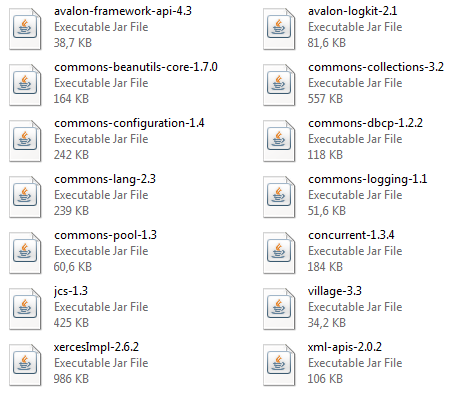
\includegraphics[height=6cm]{img/torque-lib.png}
\end{center}

\begin{lstlisting}
coches\torque-3.3\
\end{lstlisting}

\begin{center}
	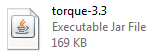
\includegraphics{img/torque-file.png}
\end{center}

Ahora ya no existen errores en el proyecto y podemos realizar una pequeña prueba de ejecución, para ello podemos crear un paquete, donde crearemos una clase Main e introduciremos el siguiente código:

\begin{lstlisting}[language=java]
import java.util.Iterator;
import java.util.List;

import org.apache.torque.Torque;
import org.apache.torque.TorqueException;
import org.apache.torque.util.Criteria;

import torque.generated.Coche;
import torque.generated.CochePeer;

public class Main 
{
	public static void main(String[] args)
	{
		/*Aqui inicializamos Torque*/
		try
		{
			Torque.init("Torque.properties");
		} 
		catch (TorqueException e) 
		{	
			e.printStackTrace();
		}
		/*Aqui probamos la conexion con la base de datos*/
		try 
		{
			Coche c = new Coche();
			c.setCocheId(3);
			c.setNombre("mondeo");
			c.save();

			Coche c1 = new Coche();
			c1.setCocheId(4);
			c1.setNombre("jumpy");
			c1.save();

		} 
		catch (Exception e) 
		{
			e.printStackTrace();
		}

		/*Aqui recuperamos los datos y los mostramos por pantalla*/
		try 
		{
			Criteria crit = new Criteria();

			List<Coche> coches = CochePeer.doSelect(crit);
			for (Iterator<Coche> i = coches.iterator(); i.hasNext();)
			{
				Coche c = (Coche) i.next();
				System.out.println("coche_id: " + c.getCocheId());
				System.out.println("nombre:  " + c.getNombre()); 
				System.out.println();
			}
		} 
		catch (TorqueException e) 
		{
			e.printStackTrace();
		}
	}
}
\end{lstlisting}

Desde nuestro main debemos de inicializar Torque, para ello hemos insertado la línea de código: 

\begin{lstlisting}[language=java]
Torque.init("Torque.properties")
\end{lstlisting}

{\bf Toque.init} toma como parámetro un fichero llamado {\bf Torque.properties}, situado en la carpeta {\bf torque-3.3}. Movemos ese archivo a la raíz del proyecto (para que sea accesible directamente), y procedemos a configurarlo. En amarillo se encuentran las líneas que han sido modificadas con respecto al archivo de configuración por defecto.

	\begin{lstlisting}
# Licensed to the Apache Software Foundation (ASF) under one
# or more contributor license agreements.  See the NOTICE file
# distributed with this work for additional information
# regarding copyright ownership.  The ASF licenses this file
# to you under the Apache License, Version 2.0 (the
# "License"); you may not use this file except in compliance
# with the License.  You may obtain a copy of the License at
#
#   http://www.apache.org/licenses/LICENSE-2.0
#
# Unless required by applicable law or agreed to in writing,
# software distributed under the License is distributed on an
# "AS IS" BASIS, WITHOUT WARRANTIES OR CONDITIONS OF ANY
# KIND, either express or implied.  See the License for the
# specific language governing permissions and limitations
# under the License.

# Directorio del proyecto
torque.applicationRoot = .

# ###########
#
#  L O G G I N G
#
# ###########
# We use Log4J for all Torque logging and we embed the log4j
# properties within our application configuration.
# ###########

# This first category is required and the category
# must be named 'default'. This is used for all logging
# where an explicit category is not specified.

# Configuraciones de logging
log4j.category.org.apache.torque = ALL, org.apache.torque
log4j.appender.org.apache.torque = org.apache.log4j.FileAppender
log4j.appender.org.apache.torque.file = ${torque.applicationRoot}/logs/torque.log
log4j.appender.org.apache.torque.layout = org.apache.log4j.PatternLayout
log4j.appender.org.apache.torque.layout.conversionPattern = %d [%t] %-5p %c - %m%n
log4j.appender.org.apache.torque.append = false

# ###########
#
#  D E F A U L T S
#
# ###########
#
# These values kick in, if you don't explicitly override them in your
# various database settings. At the moment they're only used if you
# configure the SharedPoolDataSourceFactory of the PerUserDataSourceFactory
# as your data source provider. It does not work with JNDI.
#
# The example is shown for SharedPoolDataSource.
#
# ###########

# Time to wait for a connection to the database in milliseconds.
torque.defaults.pool.maxWait = 10000

# Maximum number of idle and active connections cached in a database
# definition.
# Note that, if you have multiple database definitions which access the
# same database URL, they don't share the connections but you have
# multiple pools and each has this maximum number. So if you have a
# connection licensed database engine, you must multiply this number by
# the number of times you use a specific database URL.

torque.defaults.pool.maxIdle = 8
torque.defaults.pool.maxActive = 10

# How often the pool is checked for connection which stayed in the pool
# for too long. Defaults to 5 minutes (5 * 60 * 1000)
# remove property if the idle object evictor should not be run

torque.defaults.pool.timeBetweenEvictionRunsMillis= 300000

# Lifetime of an idle connection in the pool in milliseconds.
# Defaults to one hour (1000 * 60 * 60)

torque.defaults.pool.minEvictableIdleTimeMillis = 3600000

# Sets the driver for the data sources.
# Driver de la base de datos
torque.defaults.connection.driver = org.postgresql.Driver

# Sets the URL for the datasources

# URL de la base de datos
torque.defaults.connection.url = jdbc:postgresql://127.0.0.1:5432/coches

# Sets login and password for the data sources.

# Usuario y password para acceder a la base de datos coches
torque.defaults.connection.user = user1
torque.defaults.connection.password = user1

# ###########
#
#  T O R Q U E  P R O P E R T I E S
#
# ###########
# These are your database settings. Look in the
# org.apache.torque.pool.* packages for more information.
#
# The parameters to connect to the default database.  You MUST
# configure these properly.
# ###########

# Nombre de la base de datos
torque.database.default=coches

# Gestor de base de datos
torque.database.coches.adapter=postgresql

# # Using commons-dbcp
torque.dsfactory.coches.factory=org.apache.torque.dsfactory.SharedPoolDataSourceFactory
# torque.dsfactory.coches.factory=org.apache.torque.dsfactory.PerUserPoolDataSourceFactory
torque.dsfactory.coches.pool.maxIdle=8
torque.dsfactory.coches.pool.maxActive=10
torque.dsfactory.coches.pool.testOnBorrow=true
torque.dsfactory.coches.pool.validationQuery=SELECT 1
torque.dsfactory.coches.connection.driver = org.postgresql.Driver
torque.dsfactory.coches.connection.url = jdbc:postgresql://127.0.0.1:5432/coches
torque.dsfactory.coches.connection.user = user1
torque.dsfactory.coches.connection.password = user1

# # Using jndi
# torque.dsfactory.coches.factory=org.apache.torque.dsfactory.JndiDataSourceFactory
# torque.dsfactory.coches.jndi.path=jdbc/coches
# torque.dsfactory.coches.jndi.java.naming.factory.initial = org.apache.naming.java.javaURLContextFactory
# torque.dsfactory.coches.jndi.java.naming.factory.url.pkgs = org.apache.naming

# torque.dsfactory.coches.datasource.dataSourceName=jdbc/DBcoches
# torque.dsfactory.coches.datasource.jndiEnvironment.java.naming.factory.initial = org.apache.naming.java.javaURLContextFactory
# torque.dsfactory.coches.datasource.jndiEnvironment.java.naming.factory.url.pkgs = org.apache.naming
# torque.dsfactory.coches.datasource.maxIdle=8
# torque.dsfactory.coches.datasource.maxActive=10

# # ConnectionPoolDataSource
# torque.dsfactory.coches.factory=org.apache.torque.dsfactory.JndiDataSourceFactory
# torque.dsfactory.coches.jndi.path=jdbc/DBcoches
# torque.dsfactory.coches.jndi.java.naming.factory.initial = org.apache.naming.java.javaURLContextFactory
# torque.dsfactory.coches.jndi.java.naming.factory.url.pkgs = org.apache.naming
# torque.dsfactory.coches.datasource.classname=org.apache.commons.dbcp.cpdsadapter.DriverAdapterCPDS
# torque.dsfactory.coches.datasource.driver = org.gjt.mm.mysql.Driver
# torque.dsfactory.coches.datasource.url = jdbc:mysql://localhost:3306/torque
# torque.dsfactory.coches.datasource.user = user
# torque.dsfactory.coches.datasource.password = password

# Determines if the quantity column of the IDBroker's id_table should
# be increased automatically if requests for ids reaches a high
# volume.

torque.idbroker.clever.quantity=true

# Determines whether the managers cache instances of the business objects.
# And also whether the MethodResultCache will really cache results.

torque.manager.useCache = true
\end{lstlisting}
	
	Como último paso añadimos el driver de la base de datos a nuestro proyecto en Eclipse, situado en:
	
\begin{lstlisting}
coches\torque-gen-3.3\lib
\end{lstlisting}

\begin{center}
	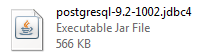
\includegraphics{img/postgresql-file.png}
\end{center}

Ya finalmente podemos ejecutar el proyecto, la salida por pantalla sería la siguiente: 
	
\begin{lstlisting}
coche_id: 3
nombre:  mondeo

coche_id: 4
nombre:  jumpy
\end{lstlisting}